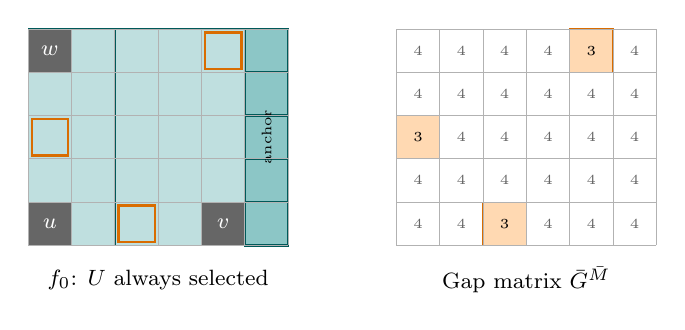
\begin{tikzpicture}[x=0.55cm,y=0.55cm]
  \tikzstyle{labelstyle}=[font=\footnotesize]
  \tikzstyle{tinylabel}=[font=\tiny]
  \tikzstyle{guidestyle}=[line width=0.3pt, draw=black!30]
  \tikzstyle{verttile}=[draw=black!70, fill=black!60, line width=0.3pt]
  \tikzstyle{keeptile}=[draw=teal!70!black, fill=teal!25, line width=0.45pt]
  \tikzstyle{anchortile}=[draw=teal!70!black, fill=teal!45, line width=0.9pt]
  \tikzstyle{midframe}=[draw=orange!85!black, fill=none, line width=0.9pt]
  \tikzstyle{midtile}=[draw=orange!85!black, fill=orange!30, line width=0.45pt]

  % body of U: the entire grid, extended by the anchor column (right) that no vertex polyomino uses
  \foreach \x in {0,...,5} {
    \foreach \y in {0,...,4} {
      \draw[keeptile] (\x,\y) rectangle ++(1,1);
    }
  }
  % anchor column: covered by U alone
  \foreach \y in {0,...,4} {
    \draw[anchortile] (5,\y) rectangle ++(1,1);
  }
  \node[tinylabel, rotate=90] at (5.5,2.5) {anchor};
  % midpoint tiles (part of U; outlined for continuity)
  \foreach \x/\y in {2/0,0/2,4/4} {
    \draw[midframe] (\x+0.08,\y+0.08) rectangle ++(0.84,0.84);
  }
  % vertex tiles (marked for orientation)
  \foreach \x/\y/\n in {0/0/u,4/0/v,0/4/w} {
    \draw[verttile] (\x,\y) rectangle ++(1,1);
    \node[labelstyle, text=white] at (\x+0.5,\y+0.5) {$\n$};
  }
  \draw[guidestyle, step=1] (0,0) grid (6,5);
  \node[labelstyle] at (3,-0.8) {$f_0$: $U$ always selected};

  % gap matrix: midpoints keep gap n = 3, all other tiles (anchor column included) get gap N = 4
  \begin{scope}[shift={(8.5,0)}]
    \foreach \x/\y in {2/0,0/2,4/4} {
      \draw[midtile] (\x,\y) rectangle ++(1,1);
      \node[tinylabel] at (\x+0.5,\y+0.5) {$3$};
    }
    \foreach \x/\y in {0/0,1/0,3/0,4/0,5/0,
                       0/1,1/1,2/1,3/1,4/1,5/1,
                       1/2,2/2,3/2,4/2,5/2,
                       0/3,1/3,2/3,3/3,4/3,5/3,
                       0/4,1/4,2/4,3/4,5/4} {
      \node[tinylabel, text=black!60] at (\x+0.5,\y+0.5) {$4$};
    }
    \draw[guidestyle, step=1] (0,0) grid (6,5);
    \node[labelstyle] at (3,-0.8) {Gap matrix $\bar{G}^{\bar{M}}$};
  \end{scope}
\end{tikzpicture}
